\documentclass[pdf]{beamer}

% select the theme using in this paper
\mode<presentation>{\usetheme{Warsaw}}

\title{Learn Beamer for \LaTeX}
\subtitle{忙里偷闲}
\author{smh}


\usepackage{xeCJK}
\setmainfont{Times New Roman}
\setCJKmainfont[BoldFont={SimHei},ItalicFont={KaiTi}]{SimSun}
\setCJKsansfont{SimHei}
\setCJKmonofont{SimSun}

\usepackage{graphicx}
\usepackage{subfigure}
\usepackage{xcolor}

\usepackage{algorithm}
\usepackage{algorithmicx}
\usepackage{algpseudocode}

\usepackage{amsmath}

\usepackage{booktabs}
\usepackage{multirow}

%\usepackage[colorlinks]{hyperref}    % beamer already loads hyperref internally

\begin{document}

\frame[plain]{\titlepage}   % use plain to custom the title page

%\begin{frame}
%\titlepage
%\end{frame}

% add table of contents to each section
\AtBeginSection[]
{
	\begin{frame}{Table of contents}
		\tableofcontents[                     % show, shared, hide
		sectionstyle=show/show,               % section=<current section>/<other section>
		subsectionstyle=show/show/show        % subsectionstyle=<current subsection>/<other subsection in current section>/<other subsection in other section>
		]
	\end{frame}
	
	\begin{frame}{Table of Contents}
			\tableofcontents[
			currentsection,
			%sectionstyle=show/show,
		%	subsectionstyle=show/show/show
			]
	\end{frame}
}

\section{Intro to Beamer}

\subsection{About Beamer 0}
\begin{frame}{What is Beamer}
The body of the frame.
\end{frame}

\subsection{Basic Structure}
\begin{frame}
Here is a well-known formula:
\begin{displaymath}
\sum_{k=0}^{n}k = \frac{n(n+1)}{2}
\end{displaymath}
\pause
\begin{itemize}
\item Here is less well-known, but still useful formula:
\begin{displaymath}
\sum_{k=0}^{n}k^2 = \frac{n(n+1)(2n+1)}{6}
\end{displaymath}
\end{itemize}
\end{frame}

\subsection{Examples}
\begin{frame}
Watch this silde below:
\begin{itemize}
\item<2->Hello, World.
\item<3->Hello, mars.
\item<4->Hello, Alpha Centauri.
\end{itemize}
\end{frame}

\section{Overlaying Concepts}


\subsection[Examples]{Examples: Lists, Graphics, Tables}
\begin{frame}
\frametitle{Lists}
Which President said ...
\begin{enumerate}[A]
\item<2-5>James Madison
\item<3-5>Harry Truman
\item<4-> \color<6>[rgb]{0,0.6,0} Abraham Lincoln      % only show this item after the 5th step !!!
\item<5-5> Calvin Coolidge
\end{enumerate}
\uncover<1-5>{Hints:}\\                        % show from the 1th step to 5th stop
\uncover<2-5>{James Madison ate broccoli.}\\   % show from the 2th step to 5th step 
\uncover<3-5>{Harry Truman drank milk.}\\
\uncover<4-5>{Abe Lincoln raised bees.}\\
\uncover<5-5>{And Cal Coolidge grew silk.}
\end{frame}


\begin{frame}
\frametitle{Graphics}
\begin{columns}
\column{0.5\textwidth}
\begin{figure}[ht]
\centering
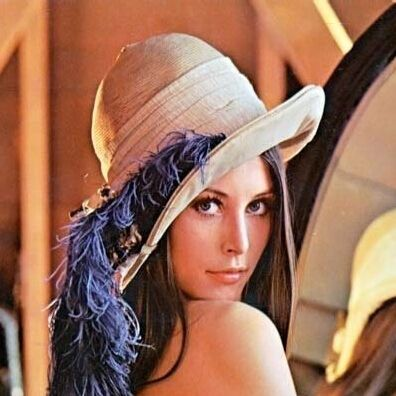
\includegraphics[height=2in]{lena}
\footnote{lena}
\end{figure}
\column{0.5\textwidth} 
\begin{block}<2->{Observation 1}        % from the 2th step to the end of this slide
Simmons Hall is composed of metal and concrete.
\end{block}
\begin{block}<3->{Observation 2}
Simmons Dormitory is composed of brick.
\end{block}
\begin{block}<4->{Conclusion}
Simmons Hall $ \not = $ Simmons Dormitory.
\end{block}
\end{columns}
\end{frame}

% new theorem must be putted outside of 'frame'
\newtheorem{thm}{Easy Theorem}
\newtheorem{pf}{Proof}
\newtheorem{rmk}{Remark}

\begin{frame}
\frametitle{Math Stuff: Backstage}

\begin{thm}<1->
$$x^n + y^n = z^n$$ 
has no integer sulutioins for $n>2$ where $x, y, z, \neq 0 $.
\end{thm}
\begin{pf}<3->
The proof is trivial and left as an exercise.
\end{pf}
\begin{rmk}<2->
This problem was first posed in $10000$ B.C.
\end{rmk}
\end{frame}

\begin{frame}
\frametitle{Building Tables}

\begin{table}[bt]
\begin{tabular}{|l|c|c|} \hline
\textbf{Ice Cream Store} & \textbf{Location} & \textbf{How to Get There} \\ 
\hline
\uncover<2->{Toscanini's} & \uncover<2->{Central Square} & \uncover<2->{Just walk!} \\
\hline
\uncover<3->{Herrell's}   & \uncover<3->{Harvard Square} & \uncover<3->{Red Line}\\
\hline
\end{tabular}
\end{table}

\end{frame}


\end{document}
